%%% Laboratory	 Notes
%%% Template by Mikhail Klassen, April 2013
%%% Contributions from Sarah Mount, May 2014
\documentclass[a4paper]{tufte-handout}

\newcommand{\workingDate}{\textsc{May $|$ 2014}}
\newcommand{\userName}{Your Name}
\newcommand{\institution}{Your University}

\usepackage{lab_notes}

\usepackage{hyperref}
\hypersetup{
    pdffitwindow=false,            % window fit to page
    pdfstartview={Fit},            % fits width of page to window
    pdftitle={Lab notes 2014},     % document title
    pdfauthor={Your Name},         % author name
    pdfsubject={},                 % document topic(s)
    pdfnewwindow=true,             % links in new window
    colorlinks=true,               % coloured links, not boxed
    linkcolor=DarkScarletRed,      % colour of internal links
    citecolor=DarkChameleon,       % colour of links to bibliography
    filecolor=DarkPlum,            % colour of file links
    urlcolor=DarkSkyBlue           % colour of external links
}


\title{Lab Notes Template}
\date{2014}

\begin{document}
\maketitle

%%%%%%%%%%%%%%%%%%%%%%%%%%%%%%%%%%%%%%%%%%%%%%%%%%%%%%%%

\begin{projects}
	\begin{description}
		\item [Alice Smith] joint work on software on low power platforms\footnote{names and ideas changd to protect the innocent}
		\item [Bob Jones] joint work on novel concurrency primitives
	\end{description}
\end{projects}

%%%%%%%%%%%%%%%%%%%%%%%%%%%%%%%%%%%%%%%%%%%%%%%%%%%%%%%%

\begin{maybe}
    \begin{itemize}
    	\item Reimplement the ideas from the paper \textit{Getting Reference Counting Back in the Ring} \citep{Shahriyar+12}
    \end{itemize}
\end{maybe}

%%%%%%%%%%%%%%%%%%%%%%%%%%%%%%%%%%%%%%%%%%%%%%%%%%%%%%%%

\newday{10 June 2014}

The (very fast) OCaml to Javascript compiler described in \citep{VouillonBalat13}\footnote{\url{http://ocsigen.org/js_of_ocaml/}} takes the unusual approach of compiling OCaml \textit{bytecode} to Javascript, rather than performing a source-to-source translation.  

\hrulefill

%%%%%%%%%%%%%%%%%%%%%%%%%%%%%%%%%%%%%%%%%%%%%%%%%%%%%%%%

\newday{9 June 2014}

Poor benchmark results. Ideas for improvement are listed in the issue tracker in the repository.

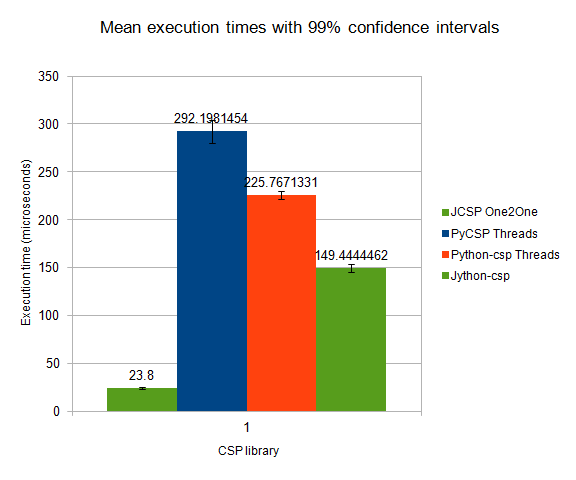
\includegraphics[scale=0.65]{benchmark}

\hrulefill

%%%%%%%%%%%%%%%%%%%%%%%%%%%%%%%%%%%%%%%%%%%%%%%%%%%%%%%%

\newday{6 June 2014}

Back from vacation.

\newthought{Student project idea} improve \url{https://github.com/snim2/Terminus} by adding new BASH commands.

Size of data sets for the ngram paper are shown in Table \ref{tab:ngram-sizes}.

\begin{table}[p]
\label{tab:ngram-sizes}
\centering
\caption{Data sizes in Google ngram data} 
\begin{tabular}{lrr} 
\toprule
Data 	&	Rows &	Compressed Size (GB)\\
\midrule
English\\
\midrule
1 gram &	472,764,897 &	4.8\\
2 gram &	6,626,604,215 &	65.6\\
3 gram &	23,260,642,968 &	218.1\\
4 gram &	32,262,967,656 &	293.5\\
5 gram &	24,492,478,978 &	221.5\\
\textbf{Totals} &	87,115,458,714 &	803.5\\
\midrule
English One Million\\
\midrule
1 gram &	261,823,186 &	2.6\\
2 gram &	3,383,379,445 &	32.1\\
3 gram &	10,565,828,499 &	94.8\\
4 gram &	12,987,703,773 &	113.1\\
5 gram &	8,747,884,729 &	75.8\\
\textbf{Totals} &	35,946,619,632 &	318.4\\
\midrule
American English\\
\midrule
1 gram &	291,639,822 &	3\\
2 gram &	3,923,370,881 &	38.3\\
3 gram &	12,368,376,963 &	113.9\\
4 gram &	15,118,570,841 &	135\\
5 gram &	10,175,161,944 &	90.2\\
\textbf{Totals} &	41,877,120,451 &	380.4\\
\midrule
British English\\
\midrule
1 gram &	188,660,459 &	1.9\\
2 gram &	2,000,106,933 &	19.1\\
3 gram &	5,186,054,851 &	46.8\\
4 gram &	5,325,077,699 &	46.6\\
5 gram &	3,044,234,000 &	26.4\\
\textbf{Totals} &	15,744,133,942 &	140.8\\
\midrule
English Fiction\\
\midrule
1 gram	&	191,545,012	&	2\\
2 gram	&	2,516,249,717	&	24.3\\
3 gram	&	7,444,565,856	&	68\\
4 gram	&	8,913,702,898	&	79.1\\
5 gram	&	6,282,045,487	&	55.5\\
\textbf{Totals}	& 25,348,108,970	&	228.9\\
\midrule
\textbf{Total without 1M}  &	170,084,822,077 &	1553.6\\
\textbf{Total without 1M} &  &	1.53TB\\
\textbf{Total}	& 206,031,441,709 &	1872\\
\textbf{Total}	& &	1.848TB\\
\end{tabular}
\end{table}


\hrulefill

%%%%%%%%%%%%%%%%%%%%%%%%%%%%%%%%%%%%%%%%%%%%%%%%%%%%%%%%

\newday{May 30 2014}

Useful datasets: \url{http://rs.io/2014/05/29/list-of-data-sets.html} In particular Mozilla have released a defect tracking dataset on GitHub\footnote{\url{https://github.com/ansymo/msr2013-bug_dataset}}\citep{Lamkanfi+13}.

Google NGram dataset can be found in Amazon S3\footnote{\url{http://aws.amazon.com/datasets/8172056142375670}}.

\hrulefill

%%%%%%%%%%%%%%%%%%%%%%%%%%%%%%%%%%%%%%%%%%%%%%%%%%%%%%%%

\newday{Jan 20 2013}

\textit{N.B.: The following is a sample entry from Mikhail Klassen's research diary. It is intended to be illustrative of how WriteLaTeX can be used the keep track of your research progress. Some names have been removed from this document for privacy.}

\section*{Initial conditions for the turbulent molecular cloud run}

\subsection*{Inner radius}

The density profile follows an $r^{-3/2}$ power law. To avoid a singularity at the center, an interpolation is done over a radius. This inner radius is defined in the parameter file. It should follow the prescription of a singular isothermal sphere (see Binney \& Tremaine p.305), which is also the definition of the King radius:
\begin{equation}
r_0 \equiv \sqrt{\frac{9\sigma^2}{4\pi G\rho_0}}
\end{equation}
where $\sigma$ is the velocity dispersion and could be estimated as $\sigma = \mathcal{M} c_s$, where $c_s = \sqrt{\gamma P/\rho} = \sqrt{\gamma k_B T / \mu}$ is the sound speed.

The isothermal sound speed in our simulation was estimated
\begin{equation}
c_s = \sqrt{\frac{k_b T}{\mu m_p}}
\end{equation}
I'm unsure why a factor of $\gamma$ was not included. For 30 K, this gives a sound speed of about 34000 cm/s or 0.34 km/s. At a Mach number of 5, this gives a supersonic dispersion of $\sigma$ = 1.7 km/s

This gives an inner radius of $r_0 \approx$ 1.595e17. 

\subsection*{Rotation}

Set the same ratio of rotational to gravitational energy $\beta$ as in Peters et al. 2010a. According to Goodman et al. (1993), this is given by (see equation 6):
\begin{equation}
\beta = \frac{1}{4 \pi G \rho_0} \omega^2
\end{equation}
In practice we can probably use the central density $\rho_c$ instead of determining an average density $\rho_0$. Looking at the numbers from other simulations, we could use an $\omega$ of 1.3e-14.

The link to the Goodman et al. (1993) paper:\\
{\tt http://adsabs.harvard.edu/cgi-bin/bib\_query?1993ApJ...406..528G}

We want to complete our simulation with a similar $\beta$ to check if disks form in the turbulent environment.

The $\omega$ necessary to produce a $\beta = 0.05$ would be
\begin{equation}
\omega = \sqrt{4 \pi G \rho_0 \beta} \approx 7.15\times 10^{-13}
\end{equation}
using $\rho_0 = \rho_c = 1.22\times10^{-17}$.

After testing this, however, I found that the rotation was much too fast. Perhaps using $\rho_0 = \rho_c$ was not a very good assumption at all, since $\rho_c$ is orders of magnitude larger than the average. I wrote a little Python script that sums up all the mass inside the outer radius and divides it by the total volume, defined by the outer radius. In this case, for an outer radius of $5.97402\times 10^{18}$ cm and about 1000 $\Msun$, we get an average density of $2.96415\times 10^{-21}$ g/cm$^3$, which gives us $\omega = 1.114 \times 10^{-14}$.

%\hrulefill

%%%%%%%%%%%%%%%%%%%%%%%%%%%%%%%%%%%%%%%%%%%%%%%%%%%%%%%%

%\newpage
\bibliographystyle{plain}
\bibliography{lab_notes}

\end{document}